\documentclass[dvipdfmx, fleqn]{jsarticle}
%% preamble for Numerical-structure-analysis report

\input{/Users/User/Documents/Project/TeX/preamble/mypreamble}

%% titles
\title{統計的機械学習 レポート}
\author{37-196360 \quad 森田涼介}


%% setting for listings
\newtcbinputlisting[auto counter]{\reportlisting}[3][]{%
	listing file = {#3},
	listing options = {language=python, style=tcblatex, numbers=left, numberstyle=\tiny},
	listing only,
	breakable,
	toprule at break = 0mm,
	bottomrule at break = 0mm,
	left = 6mm,
	sharp corners,
	drop shadow,
	title = Listings \thetcbcounter : \texttt{#2},
	label = #1,
	}



%% title format
\usepackage{titlesec}
\titleformat{\section}{\LARGE}{宿題\thesection}{0zw}{}
\newcommand{\sectionbreak}{\clearpage}
\titleformat{\subsection}{\Large}{\Alph{subsection})}{0zw}{}

\title{
	統計的機械学習 \\
	第八回 レポート ID: 01
	}
\author{37-196360 \quad 森田涼介}
\begin{document}
\maketitle


ある薬の効果を調べるために5人の被験者に対して実験を行った。
5人のうち4人の効果が認められた。
このとき,この薬の効果をベイズ推定によって分析する。



\subsection*{理論}

効果のある確率を\(\pi\)とおき,観測データは独立にベルヌーイ分布に従うとする。
また,事前分布は\(a,\ b \ (> 0)\)をパラメータとするベータ分布であると仮定する。
これらを式で表すと,
\begin{align}
    & p(\mathrm{data}|\pi) = \mathrm{Bernoulli}(\mathrm{data}|\pi) \\
    & p(\pi) = \mathrm{Beta}(\pi|a, b)
        = \frac{\Gamma(a+b)}{\Gamma(a) \Gamma(b)} \pi^{a-1} (1-\pi)^{b-1}
\end{align}
ここで,観測データのうち陽性のものの数を\(n_\mathrm{pos}\),
陰性のものの数を\(n_\mathrm{neg}\)とする。
\(p(\mathrm{data})\)は定数であることに注意すると,
\(\pi\)の事後分布の確率密度関数は,
\begin{align}
    p(\pi | \mathrm{data})
        & = \frac{p(\mathrm{data} | \pi) p(\pi)}{p(\mathrm{data})} \\
        & \propto p(\mathrm{data} | \pi) p(\pi) \\
        & = \pi^{n_\mathrm{pos}} \cdot (1 - \pi)^{n_\mathrm{neg}} \cdot \frac{\Gamma(a+b)}{\Gamma(a) \Gamma(b)} \pi^{a-1} (1-\pi)^{b-1} \\
        & \propto \pi^{a + n_\mathrm{pos} - 1} (1 - \pi)^{b + n_\mathrm{neg} - 1}
\end{align}
これを正規化すると,結局,事後分布は,
\begin{equation}
    p(\pi | \mathrm{data}) = \mathrm{Beta}(\pi | a + n_\mathrm{pos},\ b + n_\mathrm{neg})
\end{equation}
また,効果のある確率\(\pi\)が\(\mathrm{threshold}\)以上である確率は次式で計算できる。
\begin{equation}
    p(\pi \ge \mathrm{threshold} | \mathrm{data}) = \int_{\mathrm{threshold}}^{1} p(\pi | \mathrm{data}) \dd\pi
\end{equation}



\subsection*{結果}

事前分布\(\mathrm{Beta}(1,\ 1),\ \mathrm{Beta}(0.1,\ 0.1),\ \mathrm{Beta}(5,\ 5)\)について,
\(\pi \ge 0.5\),及び\(\pi \ge 0.8\)となる確率を,
数値積分により求める。
結果を表\ref{tab:result}にまとめる。
また,ベータ分布の形状を図\ref{fig:beta_dists}に示す。


\begin{table}
    \centering
    \caption{結果}
    \begin{tabular}{cccc}
        threshold & \(\mathrm{Beta}(1,\ 1)\) & \(\mathrm{Beta}(0.1,\ 0.1)\) & \(\mathrm{Beta}(5,\ 5)\) \\ \hline
        0.5 & 0.89 & 0.93 & 0.79 \\
        0.8 & 0.34 & 0.56 & 0.044
    \end{tabular}
    \label{tab:result}
\end{table}


\begin{figure}[H]
    \centering
    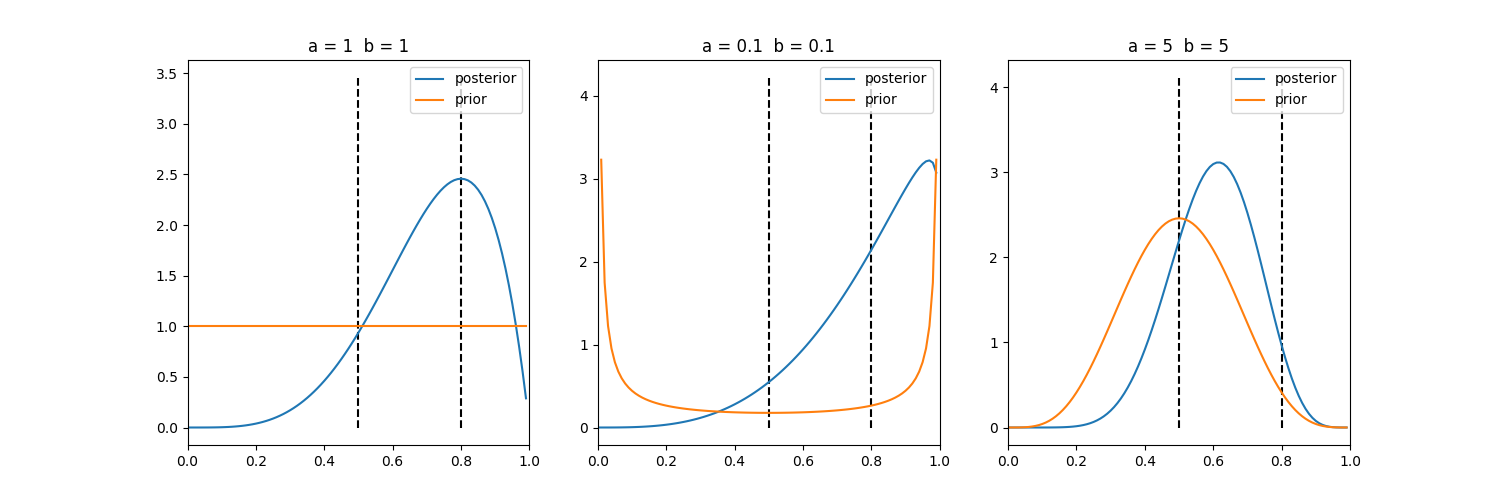
\includegraphics[clip, width=15cm]{../figures/assignment1_result}
    \caption{各\(a,\ b\)に対するベータ分布の形状}
    \label{fig:beta_dists}
\end{figure}


\subsection*{プログラム}

\reportlisting[listing:assignment1]{assignment1.py}{../program/assignment1.py}


\end{document}
